\documentclass[11pt]{article}

%===========================================================
% Packages
%===========================================================
\usepackage[margin=1in]{geometry}
\usepackage{amsmath,amssymb,bm}
\usepackage{booktabs}
\usepackage{siunitx}
\usepackage{graphicx}
\usepackage{tikz}
\usepackage{physics}
\usepackage{mathtools}
\usepackage{enumitem}
\usepackage{xcolor}
\usepackage{hyperref}
\usepackage{microtype}
\usepackage{listings}

\hypersetup{
    colorlinks=true,
    linkcolor=blue,
    citecolor=blue,
    urlcolor=blue
}

\sisetup{
    separate-uncertainty=true,
    per-mode=symbol
}

%===========================================================
% Commands
%===========================================================
\newcommand{\avg}[1]{\left\langle #1 \right\rangle}
\renewcommand{\dd}{\mathrm{d}}
\newcommand{\e}{\mathrm{e}}
\newcommand{\ii}{\mathrm{i}}
\newcommand{\SII}{\mathcal{S}_{I}}
\newcommand{\CI}{C_I}
\newcommand{\kopt}{k_0}
\newcommand{\kvec}{\mathbf{k}}
\newcommand{\rvec}{\mathbf{r}}
\newcommand{\qvec}{\mathbf{Q}}

%===========================================================
% Document
%===========================================================
\begin{document}

\begin{center}
    {\LARGE\bfseries Rotating-Diffuser Speckle as a\\
    Spatiotemporal Heating Field}

    \vspace{0.5em}

    {\large A tutorial on angular intensity, temporal autocorrelation,
    and the spectrum $\mathcal{S}_I(\mathbf{k},\omega)$}

    \vspace{1em}

    \today
\end{center}

\tableofcontents

\newpage

%===========================================================
\section{Purpose and scope}
%===========================================================

This document develops a quantitative model for light scattered from an
in-plane rotating diffuser. The intended application is a stochastic optical
heating field for thermal-transport experiments.

The primary experimental observables are:

\begin{enumerate}[label=\arabic*.]
    \item The mean scattered intensity as a function of optical scattering
    vector,
    \begin{equation}
        \overline{I}(Q).
    \end{equation}

    \item The normalized temporal intensity autocorrelation at a selected
    scattering vector,
    \begin{equation}
        g_2(Q,\tau).
    \end{equation}

    \item The spatial and temporal power spectral density of the heating
    intensity in the sample plane,
    \begin{equation}
        \SII(\kvec,\omega).
    \end{equation}
\end{enumerate}

These quantities are related, but they are not interchangeable.

In particular, knowledge of $\overline{I}(Q)$ and a collection of local
temporal autocorrelations does not, in general, determine the complete
spatiotemporal spectrum $\SII(\kvec,\omega)$. The missing information is the
correlation between different spatial positions or different optical modes.

The ideal model developed first assumes:

\begin{itemize}
    \item monochromatic coherent illumination;
    \item a thin random diffuser;
    \item a circular illuminated area of diameter $D$;
    \item illumination centered on the diffuser rotation axis;
    \item uniform illumination across that circular area;
    \item observation in the far field or a true Fourier plane;
    \item a point detector that resolves one speckle or fewer;
    \item rigid rotation of the far-field speckle pattern;
    \item statistically fully developed speckle.
\end{itemize}

Later sections discuss off-axis illumination, finite detector area, nonuniform
beams, and the distinction between rigid rotation and speckle boiling.

%===========================================================
\section{Geometry and notation}
%===========================================================

Let the optical wavelength be $\lambda$, with optical wavenumber

\begin{equation}
    \kopt = \frac{2\pi}{\lambda}.
\end{equation}

The diffuser rotates in its own plane with angular velocity

\begin{equation}
    \Omega = 2\pi f_{\mathrm{rot}},
\end{equation}

where $f_{\mathrm{rot}}$ is the rotation frequency in revolutions per second.

The incident optical wavevector is $\mathbf{k}_{\mathrm{i}}$ and the scattered
wavevector is $\mathbf{k}_{\mathrm{s}}$. The optical scattering vector is

\begin{equation}
    \qvec = \mathbf{k}_{\mathrm{s}}-\mathbf{k}_{\mathrm{i}}.
\end{equation}

For elastic scattering,

\begin{equation}
    Q = \abs{\qvec}
      = 2\kopt\sin\left(\frac{\theta}{2}\right),
    \label{eq:Q_full}
\end{equation}

where $\theta$ is the angle between the incident and scattered beams.

The transverse optical wavevector in a Fourier plane is

\begin{equation}
    Q_\perp = \kopt\sin\theta.
    \label{eq:Qtransverse}
\end{equation}

For small angles,

\begin{equation}
    Q \approx Q_\perp \approx \kopt\theta.
\end{equation}

The thermal-heating spatial frequency will be denoted by $\kvec$. This is not
the same object as the optical scattering vector $\qvec$.

\begin{quote}
\textbf{Notation warning.}
$Q$ describes the direction into which the optical field is scattered.
The vector $\kvec$ describes spatial Fourier components of the optical
\emph{intensity} pattern that heats the sample.
\end{quote}

%===========================================================
\section{Suggested optical arrangement}
%===========================================================

A simple Fourier-plane arrangement is

\begin{equation}
\text{laser}
\rightarrow
L_1
\rightarrow
\text{rotating diffuser}
\rightarrow
L_2
\rightarrow
\text{sample plane}.
\end{equation}

A nominal focal arrangement is

\begin{equation}
d(L_1,\text{diffuser})=f_1,
\qquad
d(\text{diffuser},L_2)=f_2,
\qquad
d(L_2,\text{sample plane})=f_2.
\end{equation}

A basic schematic is shown below.

\begin{center}
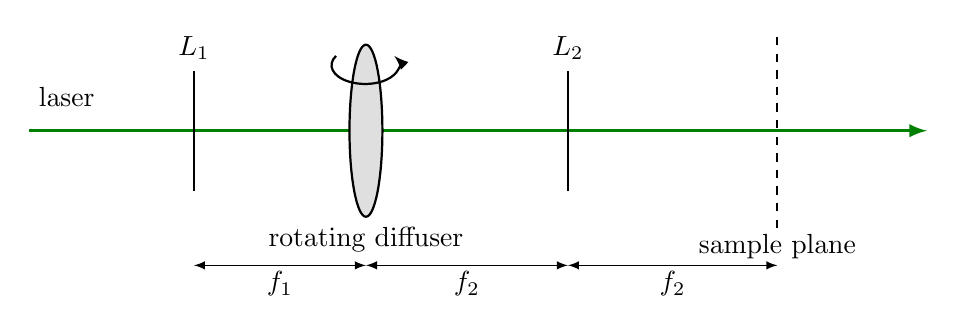
\begin{tikzpicture}[scale=0.95,>=latex]
    \draw[very thick,green!50!black,->] (-6,0)--(6,0);

    \node at (-5.5,0.45) {laser};
    \draw[thick] (-3.8,-0.8)--(-3.8,0.8);
    \node at (-3.8,1.1) {$L_1$};

    \draw[thick,fill=gray!25] (-1.5,0) ellipse (0.22 and 1.15);
    \draw[->,thick] (-1.9,1.0) arc[start angle=150,end angle=390,
                                   x radius=0.45,y radius=0.25];
    \node at (-1.5,-1.45) {rotating diffuser};

    \draw[thick] (1.2,-0.8)--(1.2,0.8);
    \node at (1.2,1.1) {$L_2$};

    \draw[dashed,thick] (4.0,-1.3)--(4.0,1.3);
    \node at (4.0,-1.55) {sample plane};

    \draw[<->] (-3.8,-1.8)--(-1.5,-1.8);
    \node at (-2.65,-2.05) {$f_1$};

    \draw[<->] (-1.5,-1.8)--(1.2,-1.8);
    \node at (-0.15,-2.05) {$f_2$};

    \draw[<->] (1.2,-1.8)--(4.0,-1.8);
    \node at (2.6,-2.05) {$f_2$};
\end{tikzpicture}
\end{center}

If the field at the sample plane is later relayed onto a camera, the relay
optics must be placed downstream of the defined sample plane. Changing the
relay magnification does not change the heating field at the sample, provided
the relay does not feed light back into the illumination system.

%===========================================================
\section{Mean angular intensity \texorpdfstring{$\overline{I}(Q)$}{I(Q)}}
%===========================================================

\subsection{Definition}

The angular scattering envelope is

\begin{equation}
    \overline{I}(Q)
    =
    \avg{I(Q,t)}_t.
\end{equation}

Experimentally, one may rotate a point detector around the diffuser or place
the detector at successive positions in a Fourier plane.

If the detector is at a physical distance $z$ from the diffuser and is
displaced laterally by $\rho$, then

\begin{equation}
    \theta = \tan^{-1}\left(\frac{\rho}{z}\right).
\end{equation}

The full optical scattering-vector magnitude is

\begin{equation}
    Q(\rho)
    =
    2\kopt
    \sin\left[
        \frac{1}{2}
        \tan^{-1}\left(\frac{\rho}{z}\right)
    \right].
\end{equation}

In a Fourier plane formed by a lens of focal length $f$,

\begin{equation}
    \rho = f\tan\theta,
\end{equation}

and therefore

\begin{equation}
    Q(\rho)
    =
    2\kopt
    \sin\left[
        \frac{1}{2}
        \tan^{-1}\left(\frac{\rho}{f}\right)
    \right].
\end{equation}

For the transverse optical wavevector,

\begin{equation}
    Q_\perp
    =
    \kopt\sin\theta
    =
    \kopt\frac{\rho}{\sqrt{f^2+\rho^2}}.
\end{equation}

For $\rho\ll f$,

\begin{equation}
    Q_\perp \approx \kopt\frac{\rho}{f}.
\end{equation}

\subsection{Count-rate normalization}

Suppose the point detector records a mean count rate
$\overline{\mathcal{R}}(\theta)$. Correct this for:

\begin{itemize}
    \item dark-count rate $\mathcal{R}_{\mathrm{dark}}$;
    \item detector quantum efficiency $\eta(\lambda)$;
    \item detector projected area;
    \item collection solid angle;
    \item polarization-dependent response;
    \item neutral-density filters;
    \item dead-time losses, if significant.
\end{itemize}

A relative angular intensity may be estimated as

\begin{equation}
    \overline{I}(Q)
    \propto
    \frac{
        \overline{\mathcal{R}}(Q)
        -
        \mathcal{R}_{\mathrm{dark}}
    }{
        \eta(\lambda)\,\Delta\Omega(Q)
    }.
\end{equation}

For a small circular detector of active diameter $d_{\mathrm{det}}$ at distance
$z$,

\begin{equation}
    \Delta\Omega
    \approx
    \frac{
        \pi d_{\mathrm{det}}^2/4
    }{z^2}.
\end{equation}

At large observation angles, the projected detector area can introduce an
additional cosine factor. It is safer to calculate the collection geometry
explicitly.

\subsection{Role of the 600-grit specification}

The nominal grit affects the angular scattering envelope
$\overline{I}(Q)$ and the microscopic statistics of the diffuser surface.

It does not appear explicitly in the ideal rigid-rotation correlation formula
derived below. In that model, the short-delay correlation width is set
principally by:

\begin{equation}
    D,\quad \lambda,\quad \Omega,\quad \theta.
\end{equation}

The actual diffuser can introduce additional boiling or loss of correlation,
which must be measured.

%===========================================================
\section{Temporal intensity autocorrelation}
%===========================================================

\subsection{Definition of \texorpdfstring{$g_2$}{g2}}

At a fixed detector coordinate or scattering angle, define

\begin{equation}
    g_2(Q,\tau)
    =
    \frac{
        \avg{I(Q,t)I(Q,t+\tau)}_t
    }{
        \avg{I(Q,t)}_t^2
    }.
    \label{eq:g2definition}
\end{equation}

Define the intensity fluctuation

\begin{equation}
    \delta I(Q,t)
    =
    I(Q,t)-\overline{I}(Q).
\end{equation}

The unnormalized covariance is

\begin{equation}
    C_I(Q,\tau)
    =
    \avg{
        \delta I(Q,t)
        \delta I(Q,t+\tau)
    }.
\end{equation}

The two are related by

\begin{equation}
    C_I(Q,\tau)
    =
    \overline{I}(Q)^2
    \left[
        g_2(Q,\tau)-1
    \right].
    \label{eq:cov_from_g2}
\end{equation}

At zero delay,

\begin{equation}
    g_2(Q,0)-1=\beta(Q),
\end{equation}

where $\beta$ is the measured speckle contrast.

For an ideal single-mode, single-polarization detector,

\begin{equation}
    \beta \rightarrow 1.
\end{equation}

Finite detector area, polarization mixing, finite time bins, and imperfect
spatial coherence reduce $\beta$.

%===========================================================
\section{Ideal centered-rotation model}
%===========================================================

\subsection{Physical picture}

Suppose a circular area of diameter $D$ is illuminated symmetrically about the
rotation axis. In the ideal Fourier-plane limit, the far-field speckle pattern
rotates rigidly with the diffuser.

At scattering angle $\theta$, two detector samples separated by diffuser
rotation angle

\begin{equation}
    \Delta\phi=\Omega\tau
\end{equation}

correspond to two points on a circle in transverse optical-wavevector space.

Their transverse separation is

\begin{equation}
    \Delta Q_\perp
    =
    2\kopt\sin\theta
    \sin\left(\frac{\Delta\phi}{2}\right).
    \label{eq:DeltaQ}
\end{equation}

For a uniformly illuminated circular aperture, the normalized field
correlation is the familiar jinc function,

\begin{equation}
    \gamma_E
    =
    \frac{2J_1(X)}{X},
\end{equation}

where

\begin{equation}
    X
    =
    \frac{D}{2}\Delta Q_\perp.
\end{equation}

Substituting Eq.~\eqref{eq:DeltaQ},

\begin{equation}
    \boxed{
    X(\theta,\tau)
    =
    \frac{2\pi D}{\lambda}
    \sin\theta
    \sin\left(\frac{\Omega\tau}{2}\right)
    }.
    \label{eq:Xexact}
\end{equation}

For fully developed Gaussian speckle, the Siegert relation gives

\begin{equation}
    \boxed{
    g_2(\theta,\tau)
    =
    1+
    \beta
    \left[
        \frac{2J_1(X)}{X}
    \right]^2
    }.
    \label{eq:g2exact}
\end{equation}

The limit at $X=0$ is understood to be

\begin{equation}
    \lim_{X\rightarrow0}\frac{2J_1(X)}{X}=1.
\end{equation}

\subsection{Short-delay form}

When

\begin{equation}
    \Omega\tau\ll1,
\end{equation}

then

\begin{equation}
    \sin\left(\frac{\Omega\tau}{2}\right)
    \approx
    \frac{\Omega\tau}{2}.
\end{equation}

Equation~\eqref{eq:Xexact} becomes

\begin{equation}
    X
    \approx
    \frac{\pi D\Omega}{\lambda}
    \sin\theta\,\tau.
    \label{eq:Xshort}
\end{equation}

Therefore,

\begin{equation}
    \boxed{
    g_2(\theta,\tau)-1
    \approx
    \beta
    \left[
        \frac{
            2J_1\left(
                \dfrac{\pi D\Omega}{\lambda}
                \sin\theta\,\tau
            \right)
        }{
            \dfrac{\pi D\Omega}{\lambda}
            \sin\theta\,\tau
        }
    \right]^2
    }.
    \label{eq:g2short}
\end{equation}

This curve is not exponential. It has an Airy-like central lobe and weak
oscillatory sidelobes.

%===========================================================
\section{Correlation-time estimates}
%===========================================================

\subsection{\texorpdfstring{$1/e$}{1/e} correlation time}

Define $\tau_{1/e}$ by

\begin{equation}
    g_2(\tau_{1/e})-1
    =
    \frac{\beta}{e}.
\end{equation}

The numerical solution of

\begin{equation}
    \left[
        \frac{2J_1(X_{1/e})}{X_{1/e}}
    \right]^2
    =
    e^{-1}
\end{equation}

is

\begin{equation}
    X_{1/e}=1.91499.
\end{equation}

Using Eq.~\eqref{eq:Xshort},

\begin{equation}
    \boxed{
    \tau_{1/e}
    =
    \frac{
        1.91499\,\lambda
    }{
        \pi D\Omega\sin\theta
    }
    }.
    \label{eq:tau1e}
\end{equation}

\subsection{First zero}

The first zero of $J_1(X)$ occurs at

\begin{equation}
    X_0=3.83171.
\end{equation}

The first zero of the ideal short-delay correlation is therefore

\begin{equation}
    \boxed{
    \tau_0
    =
    \frac{
        3.83171\,\lambda
    }{
        \pi D\Omega\sin\theta
    }
    }.
    \label{eq:tauzero}
\end{equation}

\subsection{Scaling laws}

Equations~\eqref{eq:tau1e} and \eqref{eq:tauzero} imply

\begin{equation}
    \tau_c
    \propto
    \frac{\lambda}{
        D\Omega\sin\theta
    }.
\end{equation}

Thus:

\begin{itemize}
    \item increasing illuminated diameter produces smaller far-field speckles
    and shorter point-detector correlation times;
    \item increasing rotation speed shortens the correlation time linearly;
    \item increasing detector angle shortens the correlation time through
    $\sin\theta$;
    \item at exact forward scattering, $\theta=0$, ideal rotation causes no
    decorrelation.
\end{itemize}

At $\theta=0$,

\begin{equation}
    X=0
\end{equation}

for every delay, and therefore

\begin{equation}
    g_2(0,\tau)=1+\beta.
\end{equation}

Any decay measured at exact forward scattering must come from nonideal
effects such as wobble, imperfect centering, amplitude variation, diffuser
boiling, vibration, or beam-pointing motion.

%===========================================================
\section{Numerical example}
%===========================================================

Take

\begin{align}
    \lambda &= \SI{532}{\nano\meter},\\
    D &= \SI{25}{\milli\meter},\\
    f_{\mathrm{rot}} &= \SI{1}{\hertz},\\
    \Omega &= 2\pi\ \si{\radian\per\second}.
\end{align}

Equation~\eqref{eq:tau1e} becomes

\begin{equation}
    \boxed{
    \tau_{1/e}
    =
    \frac{
        \SI{2.064}{\micro\second}
    }{
        \sin\theta
    }
    }.
\end{equation}

Equation~\eqref{eq:tauzero} becomes

\begin{equation}
    \boxed{
    \tau_0
    =
    \frac{
        \SI{4.131}{\micro\second}
    }{
        \sin\theta
    }
    }.
\end{equation}

\begin{table}[ht]
\centering
\caption{Ideal centered-illumination correlation times for a
\SI{25}{\milli\meter} illuminated diameter, \SI{532}{\nano\meter}
wavelength, and one revolution per second.}
\begin{tabular}{S[table-format=2.2]
                S[table-format=3.2]
                S[table-format=3.2]}
\toprule
{$\theta$ (degrees)}
&
{$\tau_{1/e}$}
&
{$\tau_0$}
\\
\midrule
0.01 & 11.8\,ms & 23.7\,ms\\
0.05 & 2.37\,ms & 4.73\,ms\\
0.10 & 1.18\,ms & 2.37\,ms\\
0.50 & 237\,\si{\micro\second} & 473\,\si{\micro\second}\\
1.00 & 118\,\si{\micro\second} & 237\,\si{\micro\second}\\
5.00 & 23.7\,\si{\micro\second} & 47.4\,\si{\micro\second}\\
10.0 & 11.9\,\si{\micro\second} & 23.8\,\si{\micro\second}\\
30.0 & 4.13\,\si{\micro\second} & 8.26\,\si{\micro\second}\\
60.0 & 2.38\,\si{\micro\second} & 4.77\,\si{\micro\second}\\
\bottomrule
\end{tabular}
\end{table}

The complete correlation is periodic because the same diffuser orientation
returns after every revolution:

\begin{equation}
    g_2\left(\tau+\frac{2\pi}{\Omega}\right)
    =
    g_2(\tau).
\end{equation}

For one revolution per second,

\begin{equation}
    g_2(\tau+1\ \mathrm{s})=g_2(\tau).
\end{equation}

The experiment should therefore show narrow correlation echoes at integer
multiples of the rotation period, provided the diffuser and optical alignment
remain stable.

%===========================================================
\section{Finite detector size}
%===========================================================

A detector with aperture function $A_{\mathrm{det}}(\rvec)$ measures

\begin{equation}
    I_{\mathrm{det}}(t)
    =
    \int
    A_{\mathrm{det}}(\rvec-\rvec_d)
    I(\rvec,t)
    \dd^2r.
\end{equation}

If the detector integrates over $N$ statistically independent speckles, the
contrast is approximately

\begin{equation}
    \beta\sim\frac{1}{N}.
\end{equation}

The correlation width may also broaden slightly because of spatial averaging.

For free-space propagation over distance $z$, a characteristic transverse
speckle size is

\begin{equation}
    \xi_{\mathrm{sp}}
    \sim
    \frac{\lambda z}{D}.
\end{equation}

In a Fourier plane of a lens with focal length $f$,

\begin{equation}
    \xi_{\mathrm{sp}}
    \sim
    \frac{\lambda f}{D}.
\end{equation}

A detector of active diameter $d_{\mathrm{det}}$ approximately resolves one
speckle when

\begin{equation}
    d_{\mathrm{det}}
    \lesssim
    \xi_{\mathrm{sp}}.
\end{equation}

For a \SI{20}{\micro\meter} detector, the required Fourier-plane focal length
is roughly

\begin{equation}
    f
    \gtrsim
    \frac{
        d_{\mathrm{det}}D
    }{
        \lambda
    }.
\end{equation}

For $D=\SI{25}{\milli\meter}$ and
$\lambda=\SI{532}{\nano\meter}$,

\begin{equation}
    f
    \gtrsim
    \SI{0.94}{\meter}.
\end{equation}

This estimate should be checked experimentally because definitions of speckle
diameter differ by factors of order unity.

%===========================================================
\section{Off-axis illumination}
%===========================================================

Let the beam center be displaced by radius $R$ from the diffuser rotation
axis. The local diffuser-surface speed is

\begin{equation}
    v_d=\Omega R.
\end{equation}

Off-axis illumination can produce a combination of:

\begin{itemize}
    \item rigid speckle rotation;
    \item lateral speckle translation;
    \item shear;
    \item speckle boiling;
    \item loss of exact recurrence.
\end{itemize}

There is no universal expression depending only on
$R$, $\theta$, and $\Omega$. The result also depends on:

\begin{equation}
    D,\quad
    \lambda,\quad
    \text{beam profile},\quad
    \text{diffuser statistics},\quad
    \text{ABCD optical system},\quad
    \text{detector aperture}.
\end{equation}

A practical phenomenological extension is

\begin{equation}
\boxed{
    g_2(\tau;R,\theta,\Omega)-1
    =
    \beta
    \left[
        \frac{2J_1(X)}{X}
    \right]^2
    B(\Omega R\tau)
}
\label{eq:offaxis_general}
\end{equation}

with $X$ given by Eq.~\eqref{eq:Xexact}.

A simple Gaussian model is

\begin{equation}
    B(\Omega R\tau)
    =
    \exp\left[
        -\left(
            \frac{\Omega R\tau}{\ell_R}
        \right)^2
    \right],
\end{equation}

so that

\begin{equation}
\boxed{
    g_2-1
    =
    \beta
    \left[
        \frac{2J_1(X)}{X}
    \right]^2
    \exp\left[
        -\left(
            \frac{\Omega R\tau}{\ell_R}
        \right)^2
    \right].
}
\label{eq:offaxis_gaussian}
\end{equation}

Here $\ell_R$ is an effective diffuser-displacement decorrelation length. It
must be measured rather than inferred reliably from the nominal grit.

If the additional decorrelation dominates, the corresponding time is

\begin{equation}
    \tau_R
    \sim
    \frac{\ell_R}{\Omega R}.
\end{equation}

A useful experimental test is therefore

\begin{equation}
    \tau_R^{-1}\propto\Omega R.
\end{equation}

The inferred displacement scale is

\begin{equation}
    \boxed{
    \ell_R
    =
    \Omega R\tau_R.
    }
\end{equation}

%===========================================================
\section{Temporal spectrum from the measured autocorrelation}
%===========================================================

The Wiener--Khinchin relation connects the temporal covariance and temporal
power spectral density.

At fixed $Q$,

\begin{equation}
    S_I(Q,\omega)
    =
    \int_{-\infty}^{\infty}
    C_I(Q,\tau)
    e^{-\ii\omega\tau}
    \dd\tau.
    \label{eq:temporal_WK}
\end{equation}

Using Eq.~\eqref{eq:cov_from_g2},

\begin{equation}
\boxed{
    S_I(Q,\omega)
    =
    \overline{I}(Q)^2
    \int_{-\infty}^{\infty}
    \left[
        g_2(Q,\tau)-1
    \right]
    e^{-\ii\omega\tau}
    \dd\tau.
}
\label{eq:Sfromg2}
\end{equation}

Thus, the required ingredients at each optical scattering vector are:

\begin{equation}
    \overline{I}(Q)
    \quad\text{and}\quad
    g_2(Q,\tau).
\end{equation}

The normalized $g_2$ alone gives the spectral shape but not its absolute
power. The factor $\overline{I}(Q)^2$ restores the covariance scale.

For a real stationary signal,

\begin{equation}
    C_I(Q,-\tau)=C_I(Q,\tau),
\end{equation}

so

\begin{equation}
    S_I(Q,\omega)
    =
    2
    \int_0^\infty
    C_I(Q,\tau)
    \cos(\omega\tau)
    \dd\tau.
\end{equation}

\subsection{Discrete FPGA data}

Suppose the correlator returns delays

\begin{equation}
    \tau_n=n\Delta t
\end{equation}

on a uniform grid. Compute

\begin{equation}
    C_n
    =
    \overline{I}^2
    \left[
        g_2(\tau_n)-1
    \right].
\end{equation}

A discrete cosine transform gives

\begin{equation}
    S_I(\omega_m)
    \approx
    2\Delta t
    \sum_{n=0}^{N-1}
    w_n C_n
    \cos(\omega_m\tau_n),
\end{equation}

where $w_n$ is an optional window.

For multi-tau lag spacing, the points are not uniformly spaced. Suitable
approaches are:

\begin{enumerate}[label=\arabic*.]
    \item interpolate $C_I(\tau)$ onto a uniform grid;
    \item use a nonuniform Fourier transform;
    \item fit a parametric model to $g_2$ and transform the fitted function;
    \item numerically integrate the cosine transform using the actual lag
    intervals.
\end{enumerate}

The periodic recurrence at the rotation frequency produces discrete spectral
structure at harmonics of $\Omega$ when sufficiently long acquisitions are
included.

%===========================================================
\section{The full spatial-temporal intensity spectrum}
%===========================================================

\subsection{Definition}

Let the sample-plane intensity be

\begin{equation}
    I(\rvec,t)
    =
    \overline{I}(\rvec)
    +
    \delta I(\rvec,t).
\end{equation}

For a statistically homogeneous field, define

\begin{equation}
    C_I(\Delta\rvec,\tau)
    =
    \avg{
        \delta I(\rvec,t)
        \delta I(\rvec+\Delta\rvec,t+\tau)
    }.
    \label{eq:space_time_corr}
\end{equation}

The spatiotemporal power spectral density is

\begin{equation}
\boxed{
    \SII(\kvec,\omega)
    =
    \int
    \int
    C_I(\Delta\rvec,\tau)
    e^{-\ii(\kvec\cdot\Delta\rvec-\omega\tau)}
    \dd^2(\Delta r)\,\dd\tau.
}
\label{eq:full_spectrum}
\end{equation}

Equivalently,

\begin{equation}
    C_I(\Delta\rvec,\tau)
    =
    \frac{1}{(2\pi)^3}
    \int
    \int
    \SII(\kvec,\omega)
    e^{\ii(\kvec\cdot\Delta\rvec-\omega\tau)}
    \dd^2k\,\dd\omega.
\end{equation}

The units of $\kvec$ are inverse length. The units of $\omega$ are radians per
second.

If cyclic spatial and temporal frequencies are preferred, define

\begin{equation}
    \bm{\nu}=\frac{\kvec}{2\pi},
    \qquad
    f=\frac{\omega}{2\pi}.
\end{equation}

Then $\bm{\nu}$ has units of cycles per unit length and $f$ has units of hertz.

%===========================================================
\section{Why \texorpdfstring{$\overline{I}(Q)$}{I(Q)} is not enough}
%===========================================================

The optical angular envelope $\overline{I}(Q)$ describes the average optical
power in each propagation direction.

The sample-plane optical field can be written as an angular-spectrum
superposition,

\begin{equation}
    E(\rvec,t)
    =
    \int
    A(\bm{\kappa},t)
    e^{\ii\bm{\kappa}\cdot\rvec}
    \dd^2\kappa.
\end{equation}

Here $\bm{\kappa}$ is an optical transverse wavevector.

The optical intensity is

\begin{equation}
    I(\rvec,t)
    =
    E(\rvec,t)E^*(\rvec,t).
\end{equation}

Its spatial Fourier transform is

\begin{equation}
\boxed{
    \widetilde{I}(\kvec,t)
    =
    \int
    A(\bm{\kappa},t)
    A^*(\bm{\kappa}-\kvec,t)
    \dd^2\kappa.
}
\label{eq:intensity_convolution}
\end{equation}

Thus the heating-intensity spatial spectrum is produced by differences
between pairs of optical wavevectors.

The mean angular intensity gives

\begin{equation}
    \overline{I}(Q)
    \propto
    \avg{\abs{A(\bm{\kappa},t)}^2},
\end{equation}

but Eq.~\eqref{eq:intensity_convolution} also depends on relative phases and
cross-correlations between different optical modes.

Therefore,

\begin{equation}
\boxed{
    \overline{I}(Q)
    \text{ alone does not determine }
    \SII(\kvec,\omega).
}
\end{equation}

Similarly, measuring $g_2(Q,\tau)$ at isolated detector positions gives local
temporal spectra but does not reveal correlations between different spatial
locations.

%===========================================================
\section{Ways to obtain \texorpdfstring{$\SII(\kvec,\omega)$}{S(k,omega)}}
%===========================================================

\subsection{Method 1: Camera movie at the sample plane}

This is the most direct method.

Record

\begin{equation}
    I(x,y,t_n)
\end{equation}

at the actual sample plane or at a calibrated conjugate image plane.

Subtract the temporal mean:

\begin{equation}
    \delta I(x,y,t)
    =
    I(x,y,t)
    -
    \avg{I(x,y,t)}_t.
\end{equation}

Compute the three-dimensional Fourier transform:

\begin{equation}
    \widetilde{\delta I}(k_x,k_y,\omega)
    =
    \iiint
    \delta I(x,y,t)
    e^{-\ii(k_xx+k_yy-\omega t)}
    \dd x\,\dd y\,\dd t.
\end{equation}

Then estimate

\begin{equation}
\boxed{
    \SII(k_x,k_y,\omega)
    =
    \frac{1}{A T}
    \abs{
        \widetilde{\delta I}(k_x,k_y,\omega)
    }^2.
}
\label{eq:periodogram}
\end{equation}

Here $A$ is the analyzed image area and $T$ is the acquisition duration.

In practice:

\begin{enumerate}[label=\arabic*.]
    \item subtract the camera dark frame;
    \item correct pixel gain if necessary;
    \item subtract the time-averaged image;
    \item apply spatial and temporal windows;
    \item calculate a three-dimensional FFT;
    \item square the magnitude;
    \item average neighboring blocks or repeated acquisitions.
\end{enumerate}

\subsection{Method 2: Two-point detector correlations}

With one detector fixed at $\rvec_0$ and one detector at $\rvec$, measure

\begin{equation}
    C_I(\rvec_0,\rvec,\tau)
    =
    \avg{
        \delta I(\rvec_0,t)
        \delta I(\rvec,t+\tau)
    }.
\end{equation}

If the field is homogeneous,

\begin{equation}
    C_I(\rvec_0,\rvec,\tau)
    =
    C_I(\rvec-\rvec_0,\tau).
\end{equation}

Scanning $\rvec$ reconstructs Eq.~\eqref{eq:space_time_corr}, whose Fourier
transform gives $\SII(\kvec,\omega)$.

A set of single-point autocorrelations measures only

\begin{equation}
    C_I(\rvec,\rvec,\tau).
\end{equation}

That is the diagonal of the full spatial covariance matrix and is
insufficient for general reconstruction.

\subsection{Method 3: Rigid-rotation model}

If the pattern is known to rotate rigidly,

\begin{equation}
    I(\rvec,t)
    =
    I_0\left(
        \mathbf{R}_{-\Omega t}\rvec
    \right),
    \label{eq:rigid_rotation}
\end{equation}

where $\mathbf{R}_{\phi}$ is a two-dimensional rotation matrix.

One static spatial image $I_0(x,y)$ then predicts the entire movie.

A synthetic sequence may be generated by rotating the measured frame through

\begin{equation}
    \phi_n=\Omega t_n.
\end{equation}

The resulting synthetic movie can be transformed using
Eq.~\eqref{eq:periodogram}.

This method is valid only if experiments show:

\begin{itemize}
    \item correlation echoes at every revolution;
    \item correlation times scaling as $1/\Omega$;
    \item minimal speckle boiling;
    \item minimal vibration and wobble;
    \item reproducible spatial patterns after each revolution.
\end{itemize}

%===========================================================
\section{Structure of the spectrum for rigid rotation}
%===========================================================

Express a static pattern in polar coordinates as an angular Fourier series:

\begin{equation}
    I_0(r,\phi)
    =
    \sum_{m=-\infty}^{\infty}
    I_m(r)e^{\ii m\phi}.
\end{equation}

Under rigid rotation,

\begin{equation}
    I(r,\phi,t)
    =
    I_0(r,\phi-\Omega t).
\end{equation}

Therefore,

\begin{equation}
    I(r,\phi,t)
    =
    \sum_m
    I_m(r)
    e^{\ii m\phi}
    e^{-\ii m\Omega t}.
\end{equation}

The temporal frequencies are discrete:

\begin{equation}
\boxed{
    \omega_m=m\Omega.
}
\end{equation}

Thus a perfectly repeating rotating pattern is not temporally white. Its
spectrum consists of harmonics of the rotation frequency, with amplitudes
set by the angular spatial structure.

A finite observation time broadens the spectral lines. Mechanical jitter,
surface nonuniformity, and speckle boiling can produce continuous spectral
components around the harmonics.

This is an important conceptual result:

\begin{equation}
\boxed{
    \text{Rigid rotation couples spatial angular order }m
    \text{ to temporal frequency }m\Omega.
}
\end{equation}

It does not generate independent spatial and temporal frequencies.

%===========================================================
\section{Local traveling-pattern approximation}
%===========================================================

Over a small region, a rotating pattern can resemble translation:

\begin{equation}
    I(\rvec,t)
    \approx
    I_0(\rvec-\mathbf{v}t).
\end{equation}

The Fourier representation then satisfies

\begin{equation}
    \widetilde{I}(\kvec,\omega)
    \propto
    \widetilde{I}_0(\kvec)
    \delta(\omega-\kvec\cdot\mathbf{v}).
\end{equation}

The intensity power is concentrated along the ridge

\begin{equation}
\boxed{
    \omega=\kvec\cdot\mathbf{v}.
}
\end{equation}

A measured $\SII(\kvec,\omega)$ with narrow ridges indicates traveling or
advected speckle. A broad distribution at fixed $\kvec$ indicates boiling,
deformation, or additional stochastic evolution.

%===========================================================
\section{From optical intensity to absorbed heating}
%===========================================================

Let the sample absorptance be $A_{\mathrm{abs}}(\rvec)$.

For surface-localized absorption,

\begin{equation}
    P_{\mathrm{abs}}(\rvec,t)
    =
    A_{\mathrm{abs}}(\rvec)
    I(\rvec,t).
\end{equation}

For spatially uniform absorptance,

\begin{equation}
    \delta P_{\mathrm{abs}}(\rvec,t)
    =
    A_{\mathrm{abs}}
    \delta I(\rvec,t).
\end{equation}

The absorbed-power spectrum is then

\begin{equation}
    \mathcal{S}_{P}(\kvec,\omega)
    =
    A_{\mathrm{abs}}^2
    \SII(\kvec,\omega).
\end{equation}

If absorption occurs over depth $z$ with coefficient $\mu_a$,

\begin{equation}
    P_{\mathrm{abs}}(\rvec,z,t)
    =
    \mu_a I(\rvec,t)e^{-\mu_a z}.
\end{equation}

The three-dimensional heating spectrum contains the depth transform

\begin{equation}
    \widetilde{P}_{\mathrm{abs}}
    (\kvec,k_z,\omega)
    =
    \widetilde{I}(\kvec,\omega)
    \frac{\mu_a}{
        \mu_a+\ii k_z
    }.
\end{equation}

%===========================================================
\section{Connection to thermal transport}
%===========================================================

For an isotropic diffusive material with volumetric heat capacity $C$ and
thermal conductivity $\kappa$, the Fourier-domain heat equation is

\begin{equation}
    \left[
        \kappa k^2
        -
        \ii\omega C
    \right]
    \widetilde{T}(\kvec,\omega)
    =
    \widetilde{P}_{\mathrm{abs}}(\kvec,\omega).
\end{equation}

Therefore,

\begin{equation}
\boxed{
    \widetilde{T}(\kvec,\omega)
    =
    H_{\mathrm{th}}(\kvec,\omega)
    \widetilde{P}_{\mathrm{abs}}(\kvec,\omega),
}
\end{equation}

where

\begin{equation}
\boxed{
    H_{\mathrm{th}}(\kvec,\omega)
    =
    \frac{1}{
        \kappa k^2-\ii\omega C
    }.
}
\end{equation}

With thermal diffusivity

\begin{equation}
    \alpha=\frac{\kappa}{C},
\end{equation}

the characteristic diffusive relaxation rate is

\begin{equation}
    \omega_{\mathrm{th}}=\alpha k^2.
\end{equation}

The corresponding time is

\begin{equation}
    \tau_{\mathrm{th}}=\frac{1}{\alpha k^2}.
\end{equation}

If the spatial period is

\begin{equation}
    \Lambda=\frac{2\pi}{k},
\end{equation}

then

\begin{equation}
    \tau_{\mathrm{th}}
    =
    \frac{\Lambda^2}{
        4\pi^2\alpha
    }.
\end{equation}

A useful stochastic thermal experiment requires appreciable input power in
the region of $(k,\omega)$ where the sample response is sensitive to the
transport physics of interest.

%===========================================================
\section{Recommended experimental workflow}
%===========================================================

\subsection{Stage 1: Mean scattering envelope}

At fixed diffuser speed, measure

\begin{equation}
    \overline{I}(Q)
\end{equation}

over the usable angular range.

Record:

\begin{itemize}
    \item detector angle;
    \item detector distance or Fourier-plane focal length;
    \item count rate;
    \item dark count;
    \item neutral-density attenuation;
    \item detector aperture;
    \item polarization;
    \item diffuser radius and illuminated diameter.
\end{itemize}

\subsection{Stage 2: Centered temporal correlations}

Center the illuminated circular area on the diffuser rotation axis.

Measure

\begin{equation}
    g_2(\theta,\tau)
\end{equation}

at several angles and diffuser speeds.

Test the collapse

\begin{equation}
    g_2(\theta,\tau;\Omega)
    =
    F\left(
        \Omega\tau\sin\theta
    \right).
\end{equation}

Test the predicted scaling

\begin{equation}
    \tau_{1/e}^{-1}
    \propto
    D\Omega\sin\theta.
\end{equation}

\subsection{Stage 3: Rotation echoes}

Acquire correlations through at least several rotation periods.

Check whether

\begin{equation}
    g_2(nT_{\mathrm{rot}})
    \approx
    1+\beta,
\end{equation}

where

\begin{equation}
    T_{\mathrm{rot}}=\frac{2\pi}{\Omega}.
\end{equation}

Loss of echo amplitude with increasing $n$ quantifies long-term drift or
nonrepeatability.

\subsection{Stage 4: Off-axis illumination}

Repeat for several offsets $R$.

Fit Eq.~\eqref{eq:offaxis_gaussian} or another empirical decorrelation model.

Test

\begin{equation}
    \tau_R^{-1}\propto\Omega R.
\end{equation}

Determine

\begin{equation}
    \ell_R=\Omega R\tau_R.
\end{equation}

\subsection{Stage 5: Spatially resolved measurement}

Place a camera at the actual sample plane or a calibrated conjugate plane.

Use a diffuser speed low enough to avoid temporal aliasing.

Measure

\begin{equation}
    I(x,y,t)
\end{equation}

and calculate

\begin{equation}
    \SII(k_x,k_y,\omega).
\end{equation}

Then increase the speed and verify that the FPGA-measured temporal
correlations scale consistently with $\Omega$.

\subsection{Stage 6: Thermal experiment}

Replace the camera with the sample without changing the upstream heating
optics.

The measured heating spectrum should be treated as

\begin{equation}
    \mathcal{S}_P(\kvec,\omega)
    =
    A_{\mathrm{abs}}^2
    \SII(\kvec,\omega),
\end{equation}

subject to corrections for reflection, sample roughness, nonuniform
absorptance, and finite penetration depth.

%===========================================================
\section{Data-analysis pseudocode}
%===========================================================

\subsection{Temporal spectrum from FPGA correlation data}

\begin{lstlisting}[language=Matlab,
basicstyle=\ttfamily\small,
frame=single,
caption={MATLAB/Octave-style pseudocode for a temporal spectrum.}]
% Inputs:
% tau       delay times [s]
% g2        normalized intensity autocorrelation
% Imean     mean intensity or mean count rate
%
% First obtain the covariance:
C = Imean.^2 .* (g2 - 1);

% For multi-tau data, interpolate onto a uniform lag grid:
tau_uniform = linspace(min(tau), max(tau), 2^nextpow2(length(tau)));
C_uniform = interp1(tau, C, tau_uniform, 'pchip', 0);

% Optional window:
w = hann(length(C_uniform))';
Cw = C_uniform .* w;

% Construct an even covariance for a two-sided FFT:
C_two_sided = [fliplr(Cw(2:end)), Cw];

dtau = tau_uniform(2) - tau_uniform(1);
S = real(fftshift(fft(ifftshift(C_two_sided)))) * dtau;

N = length(C_two_sided);
omega = 2*pi*((-floor(N/2)):(ceil(N/2)-1))/(N*dtau);

% Retain nonnegative frequencies if desired:
keep = omega >= 0;
omega_positive = omega(keep);
S_positive = S(keep);
\end{lstlisting}

\subsection{Three-dimensional spectrum from a camera movie}

\begin{lstlisting}[language=Matlab,
basicstyle=\ttfamily\small,
frame=single,
caption={MATLAB/Octave-style pseudocode for
$\mathcal{S}_I(k_x,k_y,\omega)$.}]
% movie has dimensions Ny x Nx x Nt
% dx, dy are sample-plane pixel spacings
% dt is frame spacing

movie = double(movie);

% Subtract the time-averaged illumination:
mean_image = mean(movie, 3);
for n = 1:size(movie,3)
    movie(:,:,n) = movie(:,:,n) - mean_image;
end

% Apply separable windows:
wx = hann(size(movie,2))';
wy = hann(size(movie,1));
wt = reshape(hann(size(movie,3)), 1, 1, []);

window3 = reshape(wy, [], 1, 1) ...
        .* reshape(wx, 1, [], 1) ...
        .* wt;

movie_w = movie .* window3;

% Three-dimensional Fourier transform:
F = fftshift(fftn(movie_w));

% Periodogram estimate:
A = size(movie,1)*dy * size(movie,2)*dx;
T = size(movie,3)*dt;
S_I = abs(F).^2 / (A*T);

% Coordinate axes:
Ny = size(movie,1);
Nx = size(movie,2);
Nt = size(movie,3);

kx = 2*pi*((-floor(Nx/2)):(ceil(Nx/2)-1))/(Nx*dx);
ky = 2*pi*((-floor(Ny/2)):(ceil(Ny/2)-1))/(Ny*dy);
omega = 2*pi*((-floor(Nt/2)):(ceil(Nt/2)-1))/(Nt*dt);
\end{lstlisting}

%===========================================================
\section{Interpretive checks}
%===========================================================

The following signatures distinguish several regimes.

\subsection{Rigid rotation}

Expected observations:

\begin{equation}
    \tau_c^{-1}\propto\Omega\sin\theta,
\end{equation}

strong recurrence at each rotation period, and spectral power concentrated at
harmonics

\begin{equation}
    \omega=m\Omega.
\end{equation}

\subsection{Local translation}

Expected observations:

\begin{equation}
    \omega=\kvec\cdot\mathbf{v}
\end{equation}

in the measured $\SII(\kvec,\omega)$.

The two-point correlation peak shifts according to

\begin{equation}
    \tau_{\mathrm{peak}}
    \approx
    \frac{
        \Delta\rvec\cdot\hat{\mathbf{v}}
    }{
        v
    }.
\end{equation}

\subsection{Speckle boiling}

Expected observations include:

\begin{itemize}
    \item loss of complete recurrence after one revolution;
    \item continuous temporal broadening around rotation harmonics;
    \item faster decay than predicted by Eq.~\eqref{eq:g2exact};
    \item weak or absent displacement-dependent correlation peaks.
\end{itemize}

\subsection{Mechanical wobble or beam motion}

Expected observations include:

\begin{itemize}
    \item modulation at the fundamental rotation frequency;
    \item decay at $\theta=0$;
    \item position-dependent mean intensity;
    \item nonreproducible echo amplitude;
    \item correlations that do not collapse against $\Omega\tau$.
\end{itemize}

%===========================================================
\section{Main conclusions}
%===========================================================

For centered illumination of a uniformly illuminated circular diffuser in a
Fourier-plane geometry, the ideal temporal autocorrelation is

\begin{equation}
    g_2(\theta,\tau)
    =
    1+
    \beta
    \left[
        \frac{
            2J_1\left(
                \dfrac{2\pi D}{\lambda}
                \sin\theta
                \sin\dfrac{\Omega\tau}{2}
            \right)
        }{
            \dfrac{2\pi D}{\lambda}
            \sin\theta
            \sin\dfrac{\Omega\tau}{2}
        }
    \right]^2.
\end{equation}

For short delays,

\begin{equation}
    \tau_{1/e}
    =
    \frac{
        1.91499\,\lambda
    }{
        \pi D\Omega\sin\theta
    }.
\end{equation}

This expression reproduces the microsecond correlation-time table for a
\SI{25}{\milli\meter} illuminated diameter at one revolution per second.

The angular mean intensity $\overline{I}(Q)$ can be measured by detector-angle
scanning. At each $Q$, the temporal spectrum follows from

\begin{equation}
    S_I(Q,\omega)
    =
    \overline{I}(Q)^2
    \mathcal{F}_{\tau\rightarrow\omega}
    \left\{
        g_2(Q,\tau)-1
    \right\}.
\end{equation}

However,

\begin{equation}
    \overline{I}(Q)
    \quad\text{and}\quad
    g_2(Q,\tau)
\end{equation}

do not generally determine the complete sample-plane spectrum

\begin{equation}
    \SII(\kvec,\omega).
\end{equation}

That quantity requires a camera movie, two-point spatial correlations, or a
validated dynamical model such as rigid rotation.

A rigidly rotating pattern produces strong coupling between spatial and
temporal structure rather than independent broadband noise. In angular
harmonics,

\begin{equation}
    \omega=m\Omega.
\end{equation}

Locally translating speckle produces

\begin{equation}
    \omega=\kvec\cdot\mathbf{v}.
\end{equation}

These relations should be measured before interpreting the diffuser as a
spatiotemporally broadband heating source.

%===========================================================
\begin{thebibliography}{99}
%===========================================================

\bibitem{GoodmanSpeckle}
J. W. Goodman,
\textit{Speckle Phenomena in Optics: Theory and Applications},
2nd ed.,
SPIE Press, Bellingham, Washington, 2020.

\bibitem{GoodmanStatistical}
J. W. Goodman,
\textit{Statistical Optics},
2nd ed.,
Wiley, Hoboken, New Jersey, 2015.

\bibitem{Churnside1982}
J. H. Churnside,
``Speckle from a rotating diffuse object,''
\textit{Journal of the Optical Society of America}
\textbf{72}, 1464--1469 (1982).

\bibitem{Yoshimura1986}
T. Yoshimura,
``Rotational and boiling motion of speckles in a two-lens imaging system,''
\textit{Journal of the Optical Society of America A}
\textbf{3}, 1018--1024 (1986).

\bibitem{Marron1988}
J. C. Marron,
``Speckle from rough rotating objects,''
\textit{Applied Optics}
\textbf{27}, 4279--4283 (1988).

\bibitem{Yura1998}
H. T. Yura, B. Rose, and S. G. Hanson,
``Speckle dynamics from in-plane rotating diffuse objects in complex
ABCD optical systems,''
\textit{Journal of the Optical Society of America A}
\textbf{15}, 1167--1173 (1998).

\bibitem{George1976}
N. George and A. Jain,
``Speckle from rough, moving objects,''
\textit{Journal of the Optical Society of America}
\textbf{66}, 1182--1192 (1976).

\end{thebibliography}

\end{document}